% --------------------------------------------------------------------

\chapter[Variables and Transients]{Variable and Transient Sources in the Galaxy and Beyond}
\def\chpname{vartrans}\label{chp:\chpname}

\noindent {\it
Mike Lund, Ashish Mahabal, Stephen Ridgway, Lucianne Walkowicz, Rahul Biswas, Michelle Lochner,
Jeonghee Rho...
}

% --------------------------------------------------------------------


Confirmed leads for Stellar variability and Fast Stellar Transients:
Mike Lund, Ashish Mahabal, Stephen Ridgway, Lucianne Walkowicz

Confirmed leads for cosmological SNe: Rahul Biswas, Michelle Lochner,
Jeonghee Rho

Confirmed leads for extragalactic transients: Ashish Mahabal

Confirmed leads on rolling cadence: Stephen Ridgway

% --------------------------------------------------------------------

\section{Introduction}

The observation of variable targets investigates the time domain, and thus realizes the essence of a synoptic survey.  Variable and transient studies are all about sampling, and different types and time scales of phenomena benefit from different sampling strategies - sometimes significantly different.  Competing objectives described in this chapter are at the heart of LSST observing strategy and cadence design.

Target types are here grouped in subsections by variability characteristics, but as will be seen, this does not mean that all targets in a group require a common cadence, since the times scales may vary dramatically.  Acquiring suitable data for a wide range of time scales presents a fundamental problem for LSST, since the available $~$800 visits to a field over the survey cannot be deployed so as to usefully sample all time scales at all times.  This fact leads to the concept of a non-uniform survey, in which parts of the sky are visited more frequently part of the time.  The merits of such options must be traded against the benefits of a more uniform survey strategy.

When evaluating a particular observation or series of observations in light of how they perform for a specific science case, it may be helpful to think of metrics as lying along a continuum between discovery and characterization. Discovery requires a minimum amount of information to recognize an event or object as a candidate of interest, which necessarily involves some level of bare-bones characterization (upon which said recognition is based); rich characterization, on the other hand, implies that an event may not only be recognized as a candidate of interest, but basic properties of the event or object may be determined from the observation (e.g. including but not limited to classification of the event). The interpretation of a given metric along this continuum has implications for the subsequent action and analysis required, particularly as regards possible follow-up observations with other facilities. 


\section{Metrics for Transients and Variables}

As the science cases outlined below are grouped by temporal behavior (rather than underlying physical causes), the metrics developed to evaluate them may be generic and applicable to seemingly disparate science cases. Here, we describe metrics that are either already coded into the sims\_maf\_contrib repo or proposed. Individual subsections below should refer back to these metric descriptions.  


\subsection{Existing Metrics}

Lund et al. (2015; \url{http://arxiv.org/pdf/1508.03175.pdf}) discuss three metrics that have been incorporated into the MAF. Two of these metrics deal explicitly with time variable behavior: a) observational triplets, and b) detection of periodic variability. 

\subsubsection{Observational triplets (TripletMetric)}

This metric provides a means of evaluating whether a transient event on some timescale of interest has been detected, by testing for a sequence of three observations. The object must be detected in quiescence, followed by two subsequent detections above some threshold; this sequence of observations allows the magnitude of the change to be measured, as well as its timescale. 

This metric may be used for a variety of astrophysical phenomena, in particular transient events on variable objects (e.g. novae, stellar flares), in that it is general with respect to the amplitude of the brightness variation as well as the timescale of said change. The requirement of a detection prior to outburst does constrain it to objects that have already been detected in quiescence (in other words, not necessarily ``true'' transients), although there may be some cases where this is not the case (e.g. a supernova occurring on a previously detected galaxy). In practice, the time lapse between the first and second and second and third observations must be comparable (between 10$^2$ and 10$^5$ seconds) for discovery. This metric may be calculated for a given OpSim run and then further reduced to a histoogram in logarithmic time bins; the minimum number of bins to construct an interesting sample of objects is source-dependent. 

\subsubsection{Periodogram purity function (PeriodicMetric)}
This metric calculates the Fourier power spectral window function of each field (Roberts et al. 1987) as a means of quantifying the completeness of phase coverage for a given periodic variable. The periodogram purity is defined as 1 minus the Fourier power spectral window function; in the perfect case, all power is concentrated in a delta function at the correct frequency, and is zero elsewhere. As power ``leaks'' away from the correct frequency as a consequence of discrete, non-ideal data sampling, the periodogram becomes more structured. For the purposes of MAF metrics, which are designed to quantify performance as a single number, the periodogram purity is quantified as the minimum value away from the correct frequency. 

\subsubsection{Phase Gap Metric (PhaseGapMetric)}
Histogram of the median and maximum phase gaps achieved in all fields

\subsubsection{Period Deviation Metric (PeriodDeviationMetric)}

This metric computes the percent deviation of recovered periods from pure sine variability.

\subsubsection{Transient Metric (transientAsciiMetric)}

Calculate what fraction of transients would be detected using an ascii input file for the lightcurve.

\subsection{Proposed Metrics}

The following is a raw list of metric ideas; these need specificity and further description. 

The triplet metric may also be altered to include filter constraints, such that the triplets are drawn from a single filter or subset of filters.  

Color evolution constraint: triplets of observations in a specific color (really requirement of two triplets in multiple filters)

  2D Histogram of delta t?s between observations constituting a triplet 

FWHM of the window function (to quantify sampling)

Maximum hour angle difference 

Fraction of discoveries vs fractional duration of eclipse

Fraction of targets vs survey duration, for which the period can be determined to 5-sigma confidence

Fraction of targets vs survey duration, for which a period change of 1$\%$ can be determined with 5-sigma confidence

Histogram of median visit series length vs maximum visit spacing within the series

Number of events adequately sampled

% --------------------------------------------------------------------


% ====================================================================
%+
% NAME:
%    section-name.tex
%
% ELEVATOR PITCH:
%    Explain in a few sentences what the relevant discovery or
%    measurement is going to be discussed, and what will be important
%    about it. This is for the browsing reader to get a quick feel
%    for what this section is about.
%
% COMMENTS:
%
%
% BUGS:
%
%
% AUTHORS:
%    Phil Marshall (@drphilmarshall)  - put your name and GitHub username here!
%-
% ====================================================================

\section{Periodic Variable Stars}
\def\secname{periodicvariables}\label{sec:\secname}

\noindent{\it Author Name(s)} % (Writing team)

% This individual section will need to describe the particular
% discoveries and measurements that are being targeted in this section's
% science case. It will be helpful to think of a ``science case" as a
% ``science project" that the authors {\it actually plan to do}. Then,
% the sections can follow the tried and tested format of an observing
% proposal: a brief description of the investigation, with references,
% followed by a technical feasibility piece. This latter part will need
% to be quantified using the MAF framework, via a set of metrics that
% need to be computed for any given observing strategy to quantify its
% impact on the described science case. Ideally, these metrics would be
% combined in a well-motivated figure of merit. The section can conclude
% with a discussion of any risks that have been identified, and how
% these could be mitigated.

Some stars may be strictly periodic, or sufficiently so to be treated as such for some purposes, in which case data from different cycles can be combined according to phase to provide a more fully sampled light curve.  It is unreasonable to suppose that LSST visits will be synchronized with variable stars, and visits will occur effectively at random phases. In a 10-year survey, most periodic stars of almost any period will benefit from  excellent phase coverage in all filters. Only a very small period range close to the sidereal day will be poorly observed.  There is no reason to believe that any likely LSST observing strategy could seriously disturb good sampling of periodic variables.

Eclipsing binaries are discussed here with variable stars, as detection of eclipses is dependent on adequate sampling of the phase curve.  However, study of the  features of an eclipse, particularly one of short duration in phase, may require sampling more appropriate to the discussion of transients.

\subsection{Nearly Periodic Variables}

Stars with a drifting  period will be served well with sampling which constrains period variations frequently through the survey.  For targets with a wide range of periods, this will be most effectively accomplished with sampling that is rather uniform through the survey.  A considerable degree of uniformity is needed for many science objectives, and distribution of visits over the full survey is more important than the exact timing.

Some variable stars do not exhibit a strictly repeating light curve, and show variations in light curve structure from period to period.  For observational purposes, these targets are better described as periodic transients, discussed in a later section.


% --------------------------------------------------------------------

\subsection{Targets and Measurements}
\label{sec:keyword:targets}

\begin{center}
\begin{tabular}{| l | p{10cm} |}
\hline Periodic Variable Type & Examples of target science\\
\hline
Eclipsing binaries & Physical properties of stars, distances, ages, evolution, apsidal precession, mass transfer induced period changes, Applegate effect\\
RR Lyrae & Galactic structure, distance ladder, RR Lyrae properties\\
Cepheids & Distance ladder, cepheid properties\\
Long Period Variables & Distance ladder, LPV properties\\
Rotational Modulation & Gyrochronology, stellar activity\\
 \hline \end{tabular}
 \end{center}

These targets share the requirement for good sampling over the variation phase curve.

For each target, the coverage of the phase curve sampling will accumulate randomly, and particular measurements or discoveries will become possible at a rate that is somewhat linear with number of acquired visits (hence linearly with time in a uniform survey).

With millions of different periods, it is difficult to imagine designing the survey to optimize this sampling, but the sampling achieved can be predicted with appropriate metrics.



% --------------------------------------------------------------------

\subsection{Metrics}
\label{sec:keyword:metrics}

\begin{center}
\begin{tabular}{| p{5cm} |p{10cm} |}
\hline Metric & Description\\
\hline
Eclipsing binary discovery & Fraction of discoveries vs fractional duration of eclipse\\
Transiting exoplanets (depth dependent) & Fraction of discoveries vs fractional duration of eclipse\\
Phase gap & Histogram vs period of the median and maximum phase gaps achieved in all fields\\
Period determination (period dependent) & Fraction of targets vs survey duration, for which the period can be determined to 5-sigma confidence\\
Period variability (period dependent) & Fraction of targets vs survey duration, for which a period change of 1\% can be determined with 5-sigma confidence\\
  \hline \end{tabular}
 \end{center}

The period metrics can be based on a standard variable curve (e.g.sinusoid) of fiducial amplitude and brightness, and/or a realistic model population of a particular variable type. These metrics can be informative for science programs.  However, it is not clear that the survey strategy can or should attempt to control these metrics, as the requirements are specific to each target, and all targets benefit from a generally uniform distribution of visits.



% --------------------------------------------------------------------

\subsection{OpSim Analysis}
\label{sec:keyword:analysis}

Current simulations show for the main survey a broad uniformity of visits, with thorough randomization of visit phase per period, giving very good phase coverage with minimum phase gaps.


% --------------------------------------------------------------------

\subsection{Discussion}
\label{sec:keyword:discussion}

For periodic variable science, two cadence characteristics should be avoided:
\begin{itemize}
\item an exactly uniform spacing of visits (which is anyway virtually impossible); \
\item a very non-uniform distribution, such as most visits concentrated in a few survey years.
 \end{itemize}

A metric for maximum phase gap will guard against the possibility that a very unusual cadence might compromise the random sampling of periodic variables.

In each case, it would help to jump-start science programs if some fraction of targets had more complete measurements early in the survey.


% ====================================================================

\navigationbar


% --------------------------------------------------------------------


% ====================================================================
%+
% NAME:
%    section-name.tex
%
% ELEVATOR PITCH:
%    Explain in a few sentences what the relevant discovery or
%    measurement is going to be discussed, and what will be important
%    about it. This is for the browsing reader to get a quick feel
%    for what this section is about.
%
% COMMENTS:
%
%
% BUGS:
%
%
% AUTHORS:
%    Phil Marshall (@drphilmarshall)  - put your name and GitHub username here!
%-
% ====================================================================

\section{Non-periodic Variable Stars}
\def\secname{variables}\label{sec:\secname}

\noindent{\it Author Name(s)} % (Writing team)

% This individual section will need to describe the particular
% discoveries and measurements that are being targeted in this section's
% science case. It will be helpful to think of a ``science case" as a
% ``science project" that the authors {\it actually plan to do}. Then,
% the sections can follow the tried and tested format of an observing
% proposal: a brief description of the investigation, with references,
% followed by a technical feasibility piece. This latter part will need
% to be quantified using the MAF framework, via a set of metrics that
% need to be computed for any given observing strategy to quantify its
% impact on the described science case. Ideally, these metrics would be
% combined in a well-motivated figure of merit. The section can conclude
% with a discussion of any risks that have been identified, and how
% these could be mitigated.


Some variable star types are not strictly periodic.  These include multi-period stars, for which Fourier analysis
may be useful, but only if the underlying frequencies are at least
critically sampled.  Irregularly variable stars may have so little
repeatable structure that  neither phase stacking nor harmonic
analysis is very useful, but patterns may become evident over
observing intervals of years or decades.

Non-periodic variable stars may benefit from complete phase coverage
over a single cycle, or other time interval  of of interest, repeated
in consecutive intervals, or in intervals distributed over the survey.
Variable stars for which thorough sampling of limited duration is
required, including eruptive variables, are considered below with
transients.

Active galactic nuclei are mentioned here as well, as they may vary as transients and/or variable, in most cases with no or only weak periodicity.

% --------------------------------------------------------------------

\subsection{Targets and Measurements}
\label{sec:\secname:targets}

The class of non-periodic variables includes a heterogeneous
assortment of objects and phenomena.

\begin{center}
\begin{tabular}{| p{5cm} | p{10cm} |}
\hline Variable Type & Examples of target science\\
\hline
Long Period Variables & Pulsation modes, internal structure, evolution\\
Multimode pulsation & Pulsation mechanisms, internal structure\\
Semi-regular variables & Pulsation mechanisms, convection \\
Pulsating irregular variables & Chaotic dynamics \\
Epsilon Aurigae systems & Circumstellar material, dark companions\\
FU Ori systems & Accretion events, jets\\
Young Stellar Objects & Accretion, jets, disks, binarity, flaring, rotation, spots, magnetic phenomena\\
Active galactic nuclei & Galaxy evolution, reverberation mapping, black hole physics\\
 \hline \end{tabular}
 \end{center}

In each case, the observational challenge is to discover and then to
characterize the targets, utilizing the power of the LSST survey to
increase by orders of magnitude the number of well-studied targets
known.  Most of the targets in the table have variation time scales of
$\simeq$ 1 week or greater, and will receive sampling commensurate
with the time scale of variation under a natural LSST cadence
($\sim$800 visits over 10 years).  Where a higher sampling rate is
needed, these will need customized attention to the time scale and the
number and duration of sampled intervals. 
A detailed discussion of young stellar objects and star formation studies
in general are found in chapter \autoref{chp:galaxy}.

% --------------------------------------------------------------------

\subsection{Metrics}
\label{sec:\secname:metrics}

\begin{center}
\begin{tabular}{| p{5cm} |p{10cm} |}
\hline Metric & Description\\
\hline
Non-periodic variables & Histogram of median visit series length vs maximum visit spacing within the series\\
  \hline \end{tabular}
 \end{center}


% --------------------------------------------------------------------

\subsection{OpSim Analysis}
\label{sec:\secname:analysis}

Current simulations provide reasonable sampling ($\sim$2 samples per time constant) for variables that change brightness on a time scale of $>$1 week.  For faster variations, an enhanced sampling rate should be studied.


% --------------------------------------------------------------------

\subsection{Discussion}
\label{sec:\secname:discussion}

Special cadences offer the opportunity to extend LSST studies to non-periodic phenomena with time scales $\leq$1 week, rather than the $>$1 week that is naturally achieved with a uniform survey.


The need for contemporaneous color information has not been addressed, and needs consideration, as with novel targets and non-repeating signals, it may not be possible to infer color relations.
% ====================================================================

\navigationbar


% --------------------------------------------------------------------


% ====================================================================
%+
% NAME:
%    section-name.tex
%
% ELEVATOR PITCH:
%    Explain in a few sentences what the relevant discovery or
%    measurement is going to be discussed, and what will be important
%    about it. This is for the browsing reader to get a quick feel
%    for what this section is about.
%
% COMMENTS:
%
%
% BUGS:
%
%
% AUTHORS:
%    Phil Marshall (@drphilmarshall)  - put your name and GitHub username here!
%-
% ====================================================================

\section{Periodic Transient Events}
\label{sec:keyword} % For example, replace "keyword" with "lenstimedelays"

\noindent{\it Author Name(s)} % (Writing team)

% This individual section will need to describe the particular
% discoveries and measurements that are being targeted in this section's
% science case. It will be helpful to think of a ``science case" as a
% ``science project" that the authors {\it actually plan to do}. Then,
% the sections can follow the tried and tested format of an observing
% proposal: a brief description of the investigation, with references,
% followed by a technical feasibility piece. This latter part will need
% to be quantified using the MAF framework, via a set of metrics that
% need to be computed for any given observing strategy to quantify its
% impact on the described science case. Ideally, these metrics would be
% combined in a well-motivated figure of merit. The section can conclude
% with a discussion of any risks that have been identified, and how
% these could be mitigated.

This section is a place holder in case periodic transients deserve focus.  However, they may fit into the previous sections.

% --------------------------------------------------------------------

\subsection{Targets and Measurements}
\label{sec:keyword:targets}

Describe the discoveries and measurements you want to make for a generic  transient,
with additional comment on specific variable types which have any special requirements.

Example events:  eclipsing binary stars, exoplanet eclipses 

Now, describe their response to the observing strategy. Qualitatively,
how will the science project be affected by the observing schedule and
conditions? In broad terms, how would we expect the observing strategy
to be optimized for this science?


% --------------------------------------------------------------------

\subsection{Metrics}
\label{sec:keyword:metrics}

Quantifying the response via MAF metrics: definition of the metrics,
and any derived overall figure of merit.


% --------------------------------------------------------------------

\subsection{OpSim Analysis}
\label{sec:keyword:analysis}

OpSim analysis: how good would the default observing strategy be, at
the time of writing for this science project?


% --------------------------------------------------------------------

\subsection{Discussion}
\label{sec:keyword:discussion}

Discussion: what risks have been identified? What suggestions could be
made to improve this science project's figure of merit, and mitigate
the identified risks?


% ====================================================================



% --------------------------------------------------------------------


% ====================================================================
%+
% NAME:
%    section-name.tex
%
% ELEVATOR PITCH:
%    Explain in a few sentences what the relevant discovery or
%    measurement is going to be discussed, and what will be important
%    about it. This is for the browsing reader to get a quick feel
%    for what this section is about.
%
% COMMENTS:
%
%
% BUGS:
%
%
% AUTHORS:
%    Phil Marshall (@drphilmarshall)  - put your name and GitHub username here!
%-
% ====================================================================

\section{Transient Events}
\label{sec:keyword} % For example, replace "keyword" with "lenstimedelays"

\noindent{\it Author Name(s)} % (Writing team)

% This individual section will need to describe the particular
% discoveries and measurements that are being targeted in this section's
% science case. It will be helpful to think of a ``science case" as a
% ``science project" that the authors {\it actually plan to do}. Then,
% the sections can follow the tried and tested format of an observing
% proposal: a brief description of the investigation, with references,
% followed by a technical feasibility piece. This latter part will need
% to be quantified using the MAF framework, via a set of metrics that
% need to be computed for any given observing strategy to quantify its
% impact on the described science case. Ideally, these metrics would be
% combined in a well-motivated figure of merit. The section can conclude
% with a discussion of any risks that have been identified, and how
% these could be mitigated.

Transient events may benefit from substantial temporal sampling (matched to the time constant of the
event) with color information (perhaps contemporaneous) to support characterization and classification, obtained over the limited duration of interest.  Transient events slower than $\sim$ weeks may be adequately sampled by a uniform LSST cadence.  Faster events may require special scheduling strategies.  For some event types, LSST can only be expected to provide a discovery service, and followup will necessarily be performed elsewhere.


% --------------------------------------------------------------------

\subsection{Targets and Measurements}
\label{sec:keyword:targets}

The class of transients includes a heterogeneous assortment of objects and phenomena.

\begin{center} 
\begin{tabular}{| p{5cm} | p{10cm} |}
\hline Transient Type & Examples of target science\\
\hline
Flare stars & Flare frequency, energy, stellar age\\
Cataclysmic variables  \& novae & Interacting binaries, stellar evolution, compact objects, explosive events\\
Supernovae & SN physics, mass loss, distance scale, cosmology\\
Active galactic nuclei & Galaxy evolution, reverberation mapping, black hole physics\\
Stellar microlensing & Exoplanet statistics\\
Gamma ray bursts & Optical discovery and characterization\\
LIGO detections & Source position and characterization\\
Serendipity & Discovery and characterization\\
 \hline \end{tabular} 
 \end{center}	
 
Among the targets in this list, only AGN are likely to be sampled with sufficient resolution by a uniform LSST cadence - in fact for AGN, a challenge may be to spread visits sufficiently in time to avoid excessive seasonal gaps.
 
For very short lived phenomena (stellar flares, CV outbursts, GRBs, LIGO events) it appears that the function of LSST will be to provide discoveries and/or simple characterization.  Followup to discovery/identification, if required, will surely take place elsewhere.  
 
For events requiring intensive monitoring (stellar microlensing, exoplanet transits), the followup will certainly take place elsewhere.

Supernovae fall in an intermediate time range.  LSST will provide multiple visits in multiple filters during the typical SN duration.  This sampling may be insufficient for many (including key) science objectives.  However, a moderate, and feasible, change to LSST observing strategy, may enhance the sampling for part of the sky part of the time, greatly enhancing the usefulness of SN observations.

Serendipitous discoveries are of course harder to plan for.  An ideal transient discovery survey would include heavy coverage of all time scales. LSST will cover longer time periods well, but will have to make some choices of emphasis in coverage of shorter time-scales.



% --------------------------------------------------------------------

\subsection{Metrics}
\label{sec:keyword:metrics}

\begin{center} 
\begin{tabular}{| p{5cm} |p{10cm} |}
\hline Metric & Description\\
\hline
SNe & Number of events adequately sampled\\ 
Serendipity & Histogram of median visit series length vs maximum visit spacing within the series\\
  \hline \end{tabular} 
 \end{center}	

The metrics for SNe will be highly specialized and based on the best available understanding of SN light curve analysis and the expected event population.

The suggested metric set for serendipity is based on the simple-minded idea that a novel transient will be characterized by a band-limited, finite waveform, and that a useful observation series will consist of a series of samples extending over the duration of the event, with at least critical sampling of the fastest variations.  Since for some event durations the number of useful time series will be small, it may be useful to look not at the median length, but the median length of a subset size preselected as possibly useful (e.g. the$10^3$ longest series).

% --------------------------------------------------------------------

\subsection{OpSim Analysis}
\label{sec:keyword:analysis}

Analysis shows that current simulations provide  poor coverage in any one filter for transient events longer than a deep drilling session ($\sim$30 minutes) and shorter than $\sim$ weeks.  

Simulated performance for SN observations must be analyzed for both main survey and mini-survey (deep drilling) productivity.  It is considered that current simulated schedules give inadequate performance for SN science.



% --------------------------------------------------------------------

\subsection{Discussion}
\label{sec:keyword:discussion}

Community studies are providing improving SNe metrics, and continuing communication between the SN and LSST communities is essential to tuning the observing strategy to deliver the SN time series that are needed and possible.

Improving LSST science return for SNe will also improve sampling of all transients with similar or somewhat shorter characteristic times.  Non-uniform survey strategies (rolling cadence) can significantly improve the LSST performance for faster transients.  Interpretation of multiple filters for novel events may be powerful, or problematic, since color may be uncertain.  

Some insight into fast transients may be available from image pairs  or triples (as opposed to more complete series).  These include the pair of images in a visit - which could be useful in studying the rise time of an extremely fast event.  This includes the characteristic grouping of visits (typically 0.5 to 1.0 hour separation) planned for purposes of identifying asteroids.  It also includes fortuitous multiple sampling due to field overlap, providing additional sampling, which may be random or systematic, depending on the scheduling, on a time scale of minutes to hours.  The sampling benefits of this fortuitous overlap have not yet been investigated.




% ====================================================================



% --------------------------------------------------------------------

% \input{cosmologicalSNe}

% --------------------------------------------------------------------

% \input{extragalactictransients}

% --------------------------------------------------------------------



% ====================================================================
% commands for stand-alone printing
%\documentclass[11pt,headsepline,cleardoubleempty,twoside,openright]{scrbook}
%\usepackage{SciBook}
%\begin{document}
% ====================================================================

% ====================================================================
%+
% NAME:
%    rollingcadence.tex
%
% ELEVATOR PITCH:
%    TODO: Explain in a few sentences what the relevant discovery or
%    measurement is going to be discussed, and what will be important
%    about it. This is for the browsing reader to get a quick feel
%    for what this section is about.
%
% COMMENTS:
%
%
% BUGS:
%
%
% AUTHORS:
%    Steve Ridgway (@StephenRidgway)
%-
% ====================================================================

\section{ Rolling Cadence }
\def\secname{rolling}\label{sec:\secname}

\noindent{\it Stephen Ridgway, \ldots} % (Writing team)

% This individual section will need to describe the particular
% discoveries and measurements that are being targeted in this section's
% science case. It will be helpful to think of a ``science case" as a
% ``science project" that the authors {\it actually plan to do}. Then,
% the sections can follow the tried and tested format of an observing
% proposal: a brief description of the investigation, with references,
% followed by a technical feasibility piece. This latter part will need
% to be quantified using the MAF framework, via a set of metrics that
% need to be computed for any given observing strategy to quantify its
% impact on the described science case. Ideally, these metrics would be
% combined in a well-motivated figure of merit. The section can conclude
% with a discussion of any risks that have been identified, and how
% these could be mitigated.

With a total of ~800 visits spaced approximately uniformly over 10 years, and distributed among 6 filters,
it is not clear that LSST can offer the sufficiently dense sampling in time for study of transients with typical durations less than or $\simeq 1$week.
This is particularly a concern for key science requiring well-sampled SNIa light curves.  Rolling cadences stand out as a
general solution that can potentially enhance sampling rates by 2$\times$ or more, on some of the sky all of the time and all of the sky some of the time, while maintaining a sufficient uniformity for survey objectives that require it.

\subsection{The Uniform Cadence}

Current schedule simulations allocate visits as pairs separated by 30-60 minutes, for the purposes of identifying asteroids.  For most science purposes, the 30-60 minute spacing is too small to reveal temporal information, and a pair will constitute effectively a single epoch of measurement.  If the expected 824 (design value) LSST visits are realized as 412 pairs, and distributed uniformly over 10 observing seasons of 6 months each, the typical separation between epochs will be 4 days.   The most numerous visits will be in the {\it r} and {\it i} filters, and the repeat visit rate in either of these will be $\simeq$ 20 days.

The possibility is still open that, for asteroid identification, visits might be required as triples or quadrupoles, in which case the universal temporal sampling will be further slowed by 1.5 or 2$\times$.

Under a strict universal cadence it is not possible to satisfy a need for more frequent sample epochs.  This leads the simulations group to investigate the options opened up by reinterpreting the concept of a universal cadence.  Instead of aiming for a strategy which attempts to observe all fields ``equally'' all the time, it would allow significant deviations from equal coverage during the survey, returning to balance at the end of the survey.

Stronger divergence from a universal cadence, allowing significant inhomogeneities to remain at the end of the survey, is of course possible, but is not under investigation or discussed here.

There is currently considerable interest in the community in strategies that provide enhanced sampling over a selected area of the sky, and rotating the selected area in order to exercise enhanced sampling over all of the survey area part of the time.  The class of cadences that provides such intervals of enhanced visits, with the focus region shifting from time to time, is termed here a rolling cadence.  As a point of terminology, observing a single sky area with enhanced cadence for a period of time will be described as a ``roll''.

\subsection{Rolling Cadence Basics}

Assume a fixed number of observing epochs for each point on the sky, nominally distributed uniformly over the survey duration.  A subset of these can be reallocated to provide improved sampling of a sky region.  This will have the inevitable effects of: (1) reducing the number of epochs available for that sky region during the rest of the survey, and (2) displace observations of other sky regions during the time of the improved temporal sampling.  In short, the cadence outside the enhanced interval will be degraded.

The essential parameters of rolling cadence are: (1) the number of samples taken from the uniform cadence, and (2) the enhancement factor for the observing rate.  The LSST document 16370, ``A Rolling Cadence Strategy for the Operations Simulator'', by K. Cook and S. Ridgway,  contains more detailed discussion and analysis.

\begin{figure}
  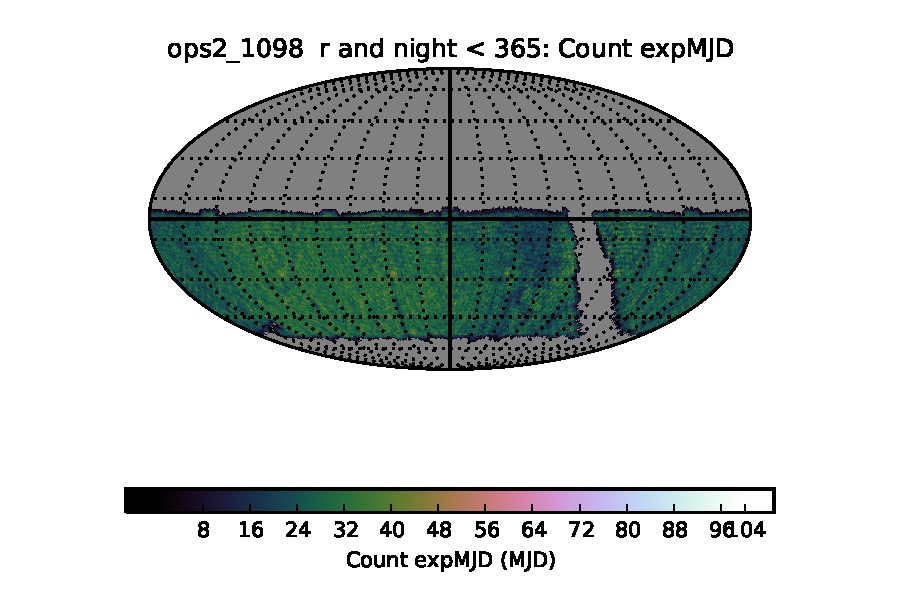
\includegraphics[width=2.3in]{figs/ops2_1098_Count_expMJD_r_and_night_lt_365_HEAL_SkyMap.pdf}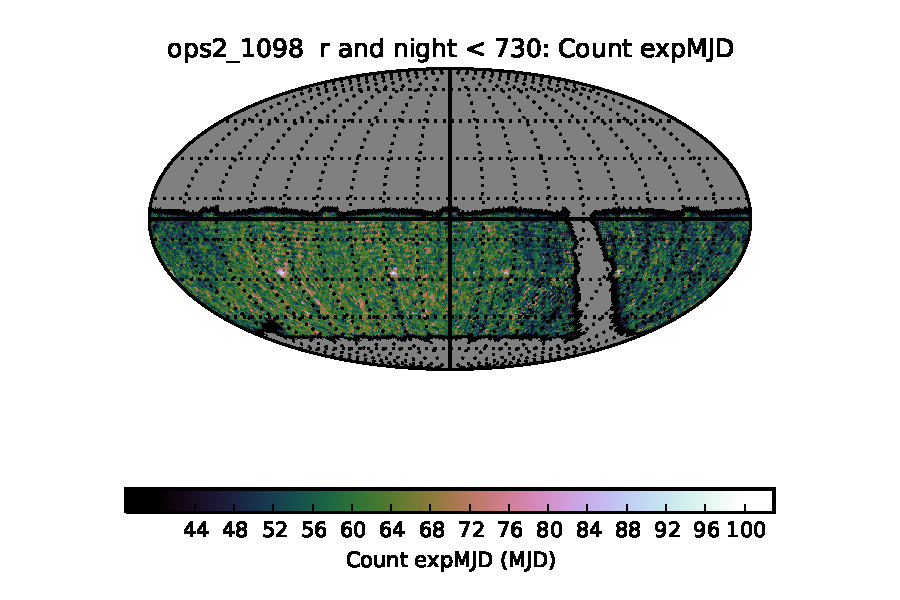
\includegraphics[width=2.3in]{figs/ops2_1098_Count_expMJD_r_and_night_lt_730_HEAL_SkyMap.pdf}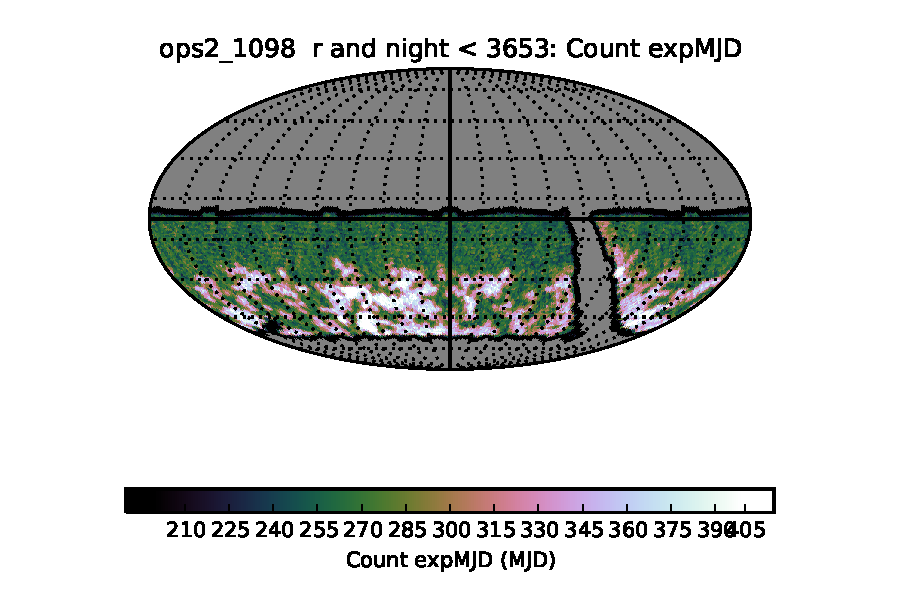
\includegraphics[width=2.3in]{figs/ops2_1098_Count_expMJD_r_and_night_lt_3653_HEAL_SkyMap.pdf} \\
  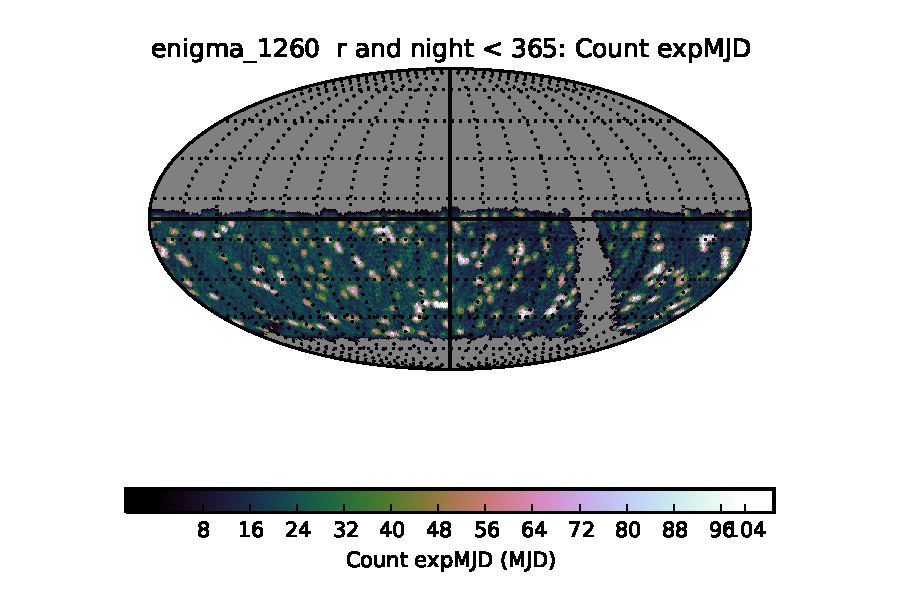
\includegraphics[width=2.3in]{figs/enigma_1260_Count_expMJD_r_and_night_lt_365_HEAL_SkyMap.pdf}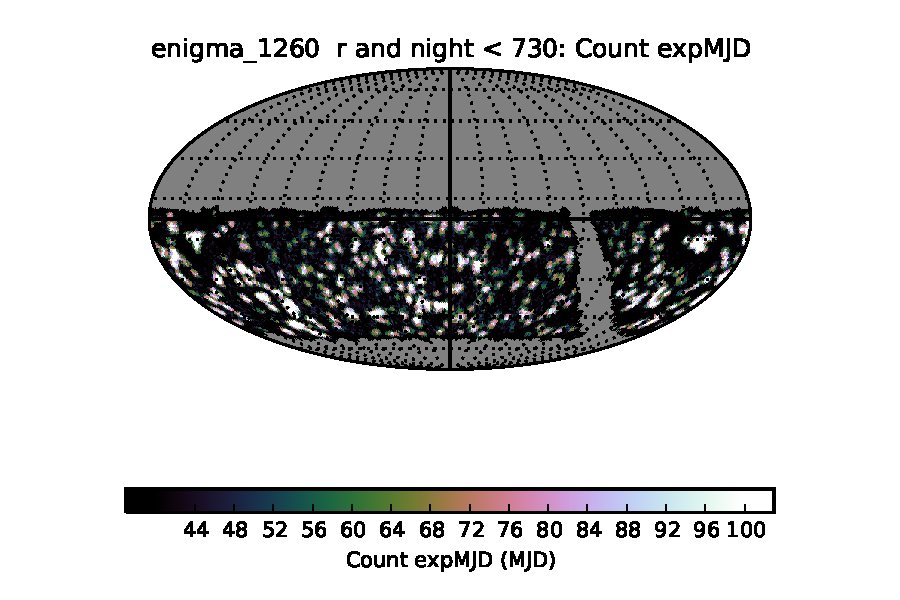
\includegraphics[width=2.3in]{figs/enigma_1260_Count_expMJD_r_and_night_lt_730_HEAL_SkyMap.pdf}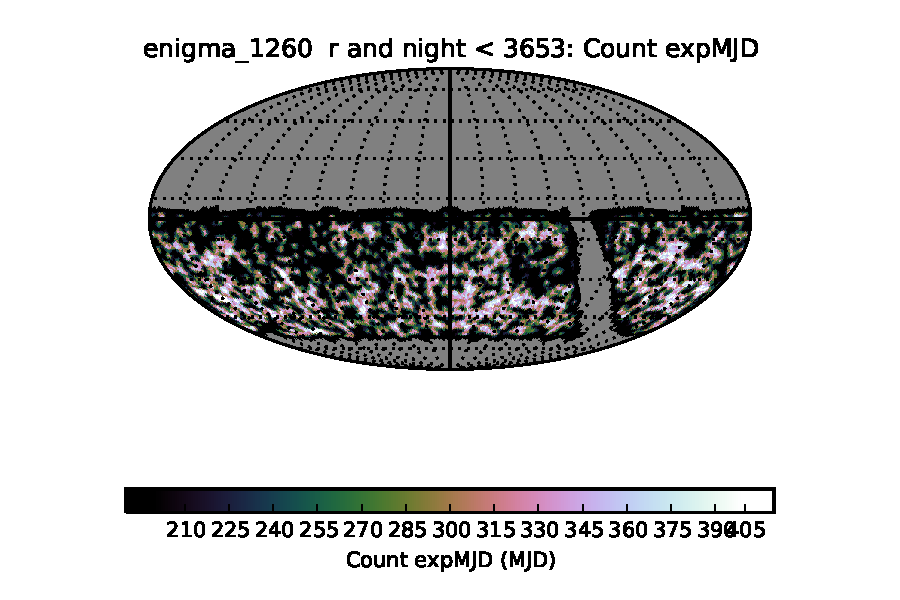
\includegraphics[width=2.3in]{figs/enigma_1260_Count_expMJD_r_and_night_lt_3653_HEAL_SkyMap.pdf}
  \caption{Example of a regular uniform survey (top) and a rolling cadence survey (bottom) after 1, 2, and 10 years in the $r$ filter.  For the regular survey, the number of visits for any part of the sky is relatively constant throughout the survey.  For the rolling cadence simulation, there are regions with many more exposures in year one which then fade in year two as other parts of the sky are emphasized.\label{fig:rollingcadence}}
\end{figure}

% --------------------------------------------------------------------
% --------------------------------------------------------------------
\subsection{ Supernovae and Rolling Cadence}
\label{sec:rolling:supernovae}

\noindent{\it Author Name(s)} % (Writing team)

Supernovae as a science topic are addressed elsewhere.
In this section, the demands of SN are used to directly constrain or
orient the rolling cadence development.

Pending more quantitative guidance, the SN objective for rolling cadence is to obtain multicolor time series significantly longer than the typical SN duration, with a cadence significantly faster than uniform.  As an example we discuss the option of a rolling cadence with the regular distribution of filters.

As a simple example, consider improving the cadence by a factor of 2 or 3.  Is we accept that some regions of the sky will be enhanced every year, and that uniform sky coverage will only arrive at the end of 10 years, then we could use, e.g., 10\% of the total epochs in a single roll.  If the enhancement is 2$\times$, each roll would last for $\simeq$ 6 months, with high efficiency for capture of complete SN events.  If the enhancement is 4$\times$, each roll would last for 2 months, with lower efficiency.

If it is important to achieve survey uniformity after 3 years, the available visits for each roll would be reduced also.  With a 2$\times$ enhancement of epoch frequency, a roll would last 2 months.

Some leverage would be gained by using more than 10\% of the available visits for a single roll.  However, this begins to impact the sampling of slow variables reduce schedule flexibility and robustness, and should be approached with caution.

From these examples, it appears that a 2$\times$ enhancement with uniformity closure after 10 years is relatively feasible and promising.  Much higher gains, or more rapid closure, require additional compromises.

% --------------------------------------------------------------------

\subsection{ Fast Transients and Rolling Cadence}
\label{sec:rolling:transients}

\noindent{\it Author Name(s)} % (Writing team)

Fast transients as a science topic are addressed elsewhere. In this section, the demands of fast transients are used to directly constrain or
orient the rolling cadence development.

By ``fast transients'', we are referring to events that are sufficiently fast that they are not addressed by the rolling cadence designed for SN observations, and slow enough that they are not covered in ``deep drilling'' type mini-surveys.  For higher tempo rolls, it is quite difficult to obtain full color data, because of the constraints on filter selection.  For this example, we will examine a rolling cadence utilizing only the {\it r} and {\it i} filters, as they are used for most visits. They are close in wavelength, and we assume that sufficient color information will be obtained by the ``background'' uniform survey that continues during a roll.

Again using 10\% of the available visits from the full 10 year survey for a single roll, we find that there would be enough epochs for each roll to acquire 1 visit per day for 21 consecutive days, giving an enhancement of 10$\times$.

Alternatively, the same epochs could be used to observe a target every 20 minutes for 12 hours during a single night (here it is assumed that visit pairs are not required, doubling the available epochs) for an enhancement of 300$\times$.

Several different possible redeployments of portions of a uniform survey have been described, each using 10\% of available time.  Of course it is possible in principal to implement multiple options, sequentially or maybe in parallel in some cases. This may pose considerable challenges to the scheduling strategy design by introducing incompatible boundary conditions.

While rolling cadences are powerful, they have limitations.  For example, sampling events that last longer than $\simeq$1 day and less than $\simeq$ 1 week have the obvious problem of diurnal availability.  In this example, intermediate cadences could be implemented in the circumpolar region, where diurnal access is much extended.  This is an example of a case in which a mini-survey of a limited number of regions could be considered as an alternative to a rolling cadence applied to the entire main survey.

% --------------------------------------------------------------------

\subsection{ Constraints, Trades and Compromises for Rolling Cadences}
\label{sec:rolling:trades}

While rolling cadences offer some attractive benefits, it is important to realize that rolling cadences are very highly constrained, and that they do bring disadvantages and compromises.

There are strong arguments against beginning a rolling cadence in the first, or even the second year of the survey.  Early in the survey, it is important to obtain for each field/filter combination, an adequate number of good quality photometric images, and at least one image in excellent seeing, to support closure of photometry reductions and to support generation of template images.

Since major science goals require a significant degree of survey homogeneity, it may be advisable to implement a strategy that brings the survey to nominal uniform depth at several times, e.g. after 3 or 5 years.  This would strongly constrain rolling cadences.

Some science objectives favor certain distributions of visits.  For astrometry, visits early and late in the survey and at large parallax factors, are beneficial.  Slow variables may benefit from uniform spacing.  Rolling cadences might impact these constraints either favorably or unfavorably.

Many objectives are served by randomization of observing conditions for each field.  Some rolling cadences could tend to reduce this randomization, for example by acquiring a large number of observations during a meteorologically favorable or unfavorable season, or during a period of instrument performance variance.

Dithering does not work gracefully with a rolling cadence, reducing temporal coverage at the boundaries of the selected sky region.  This is negligible for small dithers, but important for large dithers, which are under consideration.

These cautions illustrate that evaluation of rolling cadences must be based on the full range of schedule performance metrics, and not just those targeted by rolling cadence development.

\subsection{ Directions for Future Work with Rolling Cadences}
\label{sec:rolling:directions}

While preliminary experiments with rolling cadences have been carried out with OpSim, these experiments have signficant deficiencies, and are not suited for in-depth study as of this writing.  Progress in rolling cadence simulations is expected no sooner than mid to late-2016. Preparatory to that, analysis of cadences described above can guide development of objectives for enhancement by rolling cadence.  

Rolling cadences will be required to pass the same metrics as an other, and general requirements such as sky area, depth and visit count must be met.  Of particular interest will be metrics that clearly distinguish the gains available with rolling cadences - that is, metrics that measure schedule performance for variable targets, and especially those with strong sampling requirements, or more rapid variablity.

The following metrics, based on similar metrics developed for particular science objectives, may be useful in tuning rolling cadence performance. 

\begin{enumerate}
\item Observation Pairs histograms.  Visit pairs are simple and easy to quantify.  A pair of visits in the same filter describe a brightness change and constrain the rate of change. A visit pair in different filters (probably not coeval) constrain a color.  These metrics will describe how rapidly LSST can detect a change in the source fluxes. They will be useful for such science as early discovery of SNe, and identification of interesting galactic microlensing events.

\item Observation Triplets histograms. Similar to Pairs, but with closely spaced triplets allowing detection and confirmation of transient events (as described in http://arxiv.org/pdf/1508.03175v2.pdf).

\item Period determination metric.  Compute a measure of the period determination accuracy after a given time interval, as a function of period. A complete analysis would allow use of real light curves for various object types with realistic brightness distributions.  A simpler approach would use a single example light curve and a fixed measurement error value. A simplest approach would be based on the samping function and its power spectrum (as described in http://arxiv.org/pdf/1508.03175v2.pdf).  This metric group would rate simulation performance for period determination of periodic variables - mostly stars.

\item Sampling of SNe light curves.  The most complete metric would count the number of SNe (of various types) light curves that would be well sampled (according to defined criteria), based on analysis of realistic simulated data.  A simpler metric would be based on estimated sampling requirements and cadence without considering brightness. The latter could be used initially, pending replacement (or calibration) with more extensive simulations.

\item Time series count. For any transient or irregular variable, the optimum observational data will require multiple time and color samples within the duration of the event. Since the category of transients may include discoveries, it is not possible to exhaustively specify the source characteristics. A time series can be defined to consist of a series of samples, over some total duration T, with sampling interval t to tolerance d. The count of time series depends on the total duration, the number of samples, as well as the filter selection, so the challenge is how to visualize this information, and how to extract useful characteristic summary measures of performance.  This type of data can be valuable for identification and study of rapid phenomena such as stellar flares, binary mass transfer events, and exoplanet transits, and for slower events such as AGN reverberation mapping.

\end{enumerate}

% ====================================================================

\navigationbar

% ====================================================================
% commands for stand-alone printing
% \bibliographystyle{apj}
% \bibliography{references}
% \end{document}
% ====================================================================


% --------------------------------------------------------------------
